
\subsection{Available Superconducting Materials}

At the beginning of the \nth{20} century, Heike Kamerlingh Onnes liquified helium and started using it to cool down various metals to extremely low temperatures. He discovered that the resistance of solid mercury disappeared at $T=4.2~\text{K}$ and named this phenomenon a "superconductivity". Since that period, there have been many materials discovered, each characterised by similar physical properties corresponding to superconductivity. There are two main types of superconductors distinguished by the temperature at which they loose their superconducting state: 
\begin{itemize}
    \item Low-temperature superconductors (LTS).
    \item High-temperature superconductors (HTS).
\end{itemize}
LTS-based cables can operate in a superconducting state in the range of $T \in (4, 20)~\text{K}$ whereas HTS-based ones -- at higher temperatures than $T=20~\text{K}$. The HTS technology is very promising for future applications because it will enable machines for an operation at higher magnetic fields while spending less energy to cool it. However, the HTS cables still remain at the stage of research and development in most of the applications concerning accelerator magnets~\cite[p.~77-95]{evans_marvel_of_technology}. 

In order to use a superconductor in engineering applications for a magnet design, it~must meet four basic requirements~\cite[p.~77-95]{evans_marvel_of_technology}:

\begin{enumerate}
    \item The material should have appropriate basic physical properties, i.e. high critical temperature and critical magnetic field.
    \item The material must be relatively common, i.e. reasonably cheap.
    \item The material must be easy to form into common circular or rectangular shapes in~order to use it for the fabrication of tapes or wires.
    \item The material must withstand mechanical loads inside a magnet.
\end{enumerate}

There are two low-temperature superconductors that are commercially available for a~large scale magnet production: Nb-Ti and $\text{Nb}_3 \text{Sn}$. Each of them meets most of the specified technical requirements. Nb-Ti is an alloy widely used in a magnet design due to its ductility that allows for an easy cable extrusion and further winding process. $\text{Nb}_3 \text{Sn}$ is a brittle material sensitive to mechanical stresses. It requires a greater effort in coil production compared to Nb-Ti. In the fabrication process, it is initially formed to resemble its final geometry. The~next manufacturing step consists of a few day high-temperature treatment during which the mixture of Nb and Sn binds in order to create a superconducting compound. The main advantage of $\text{Nb}_3 \text{Sn}$ is its higher critical parameters of temperature and magnetic field with respect to Nb-Ti~\cite[p.~29-41]{superconducting_accelerator_magnets}.

\subsection{Critical Parameters and Stability}

The superconducting state depends on three critical parameters: temperature, magnetic field, and current density, as illustrated in Fig.~\ref{fig:scheme_critical_surface}. These three variables create the so called "critical surface" under which a material remains in the superconducting state. The~transition from the superconducting to the normal state is called a "quench". It occurs when an operating point of a superconductor remains outside of the critical surface. One can notice in Fig.~\ref{fig:scheme_critical_surface} that $\text{Nb}_3 \text{Sn}$ is characterised by a larger volume under the critical surface with respect to Nb-Ti. Higher critical parameters of this material allow for its potential usage at stronger fields in accelerator magnets.

\begin{figure}[H]
    \centering
    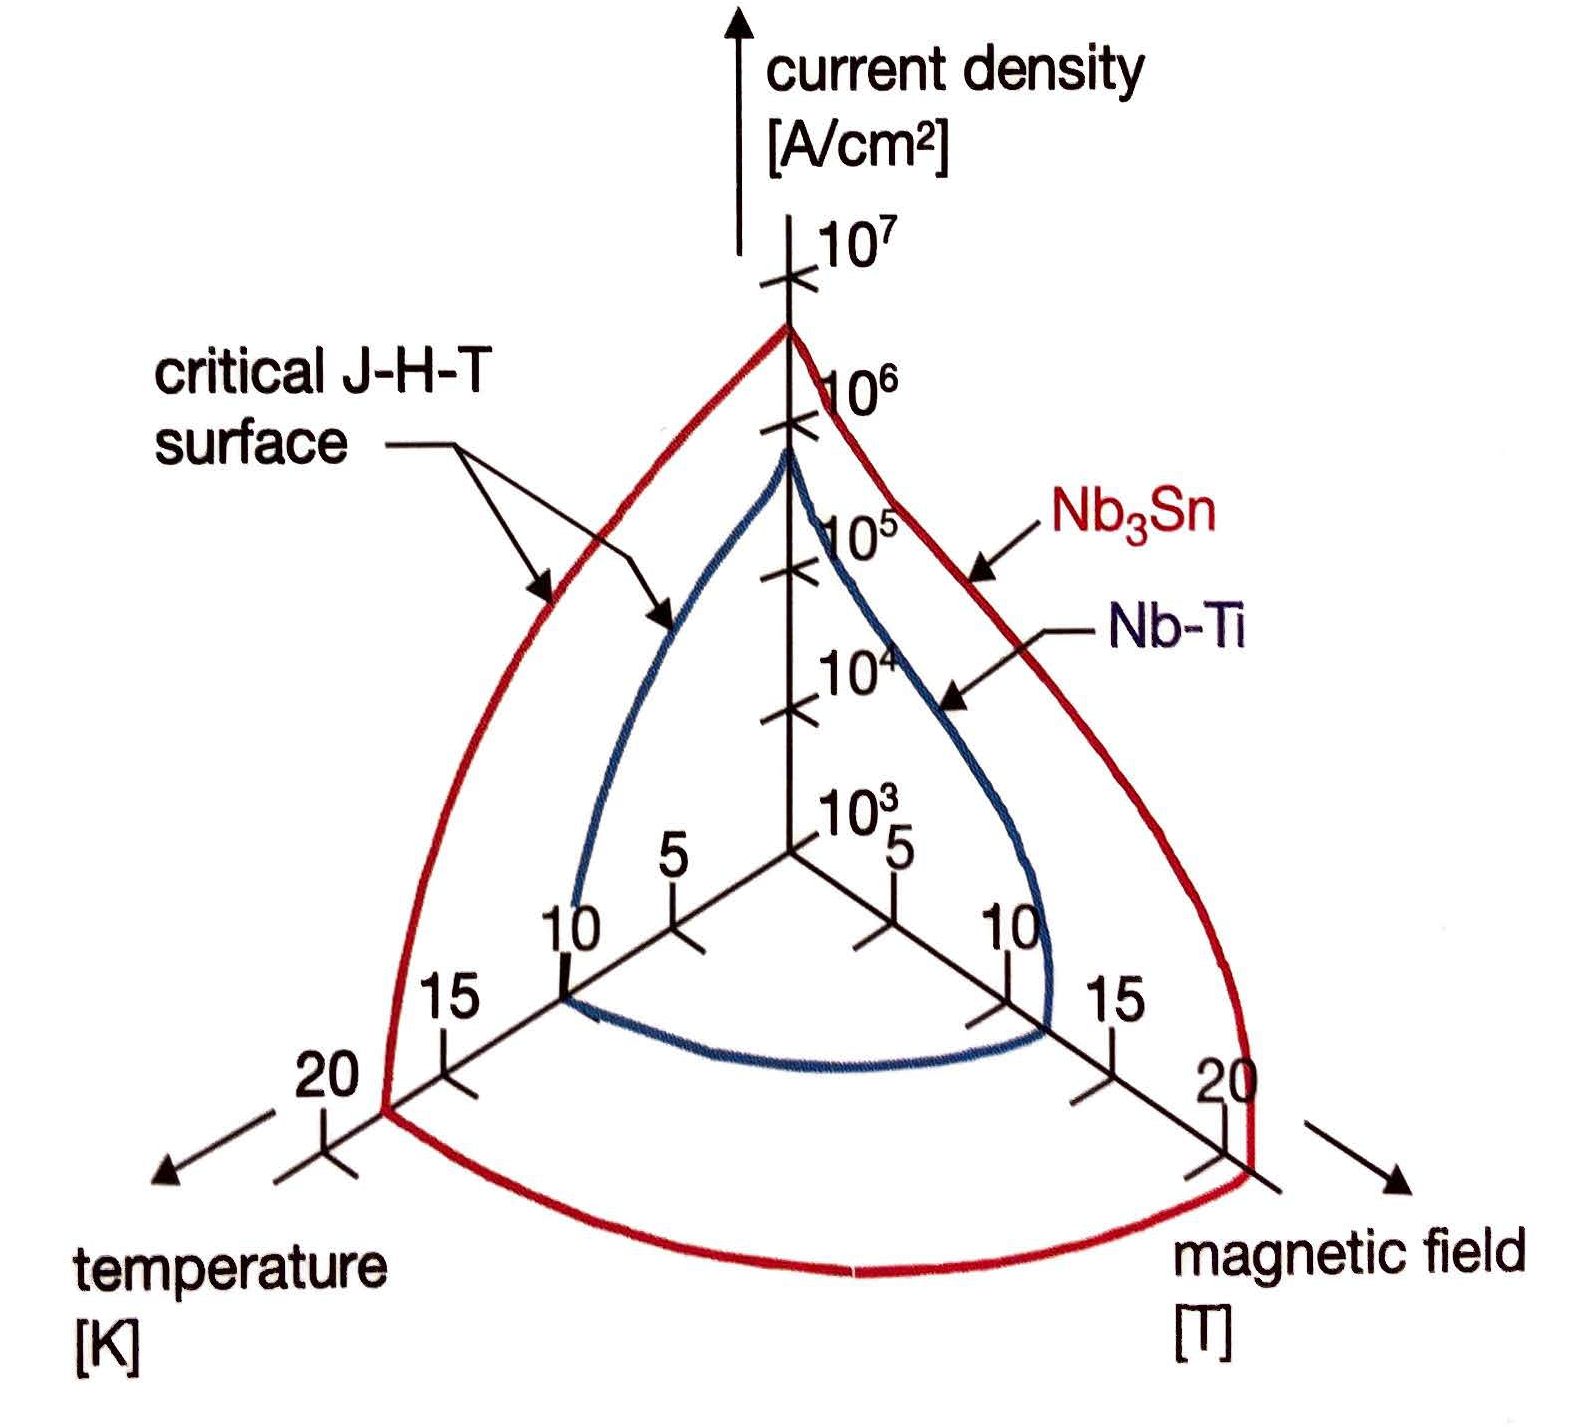
\includegraphics[width=0.35\linewidth]{sections/introduction/figures/critical_surface_scheme.png}
    \caption{Critical surface for $\text{Nb}_\text{3}\text{Sn}$ and Nb-Ti \cite{evans_marvel_of_technology}}
    \label{fig:scheme_critical_surface}
\end{figure} 

At operating temperatures of an LTS magnet, being in the range of $T \in (1.9, 4.5)~\text{K}$, even a small energy deposition in the order of $1~\frac{\text{mJ}}{g}$ may cause a quench. It is mainly due to an extreme low heat capacity of solid materials at cryogenic temperatures (see Appendix~\ref{appendix_material_properties_description}). In addition, superconductors have relatively high resistivity in a normal conducting state with respect to the materials considered to be good electrical conductors such as copper. As described in Fig.~\ref{fig:resitivity_tin_copper}, the resistivity of tin, being a superconductor below $T_\text{c}$, is higher at the normal conducting state with respect to copper~\cite[p.~1-6]{superconducting_accelerator_magnets}.

\begin{figure}[H]
    \centering
    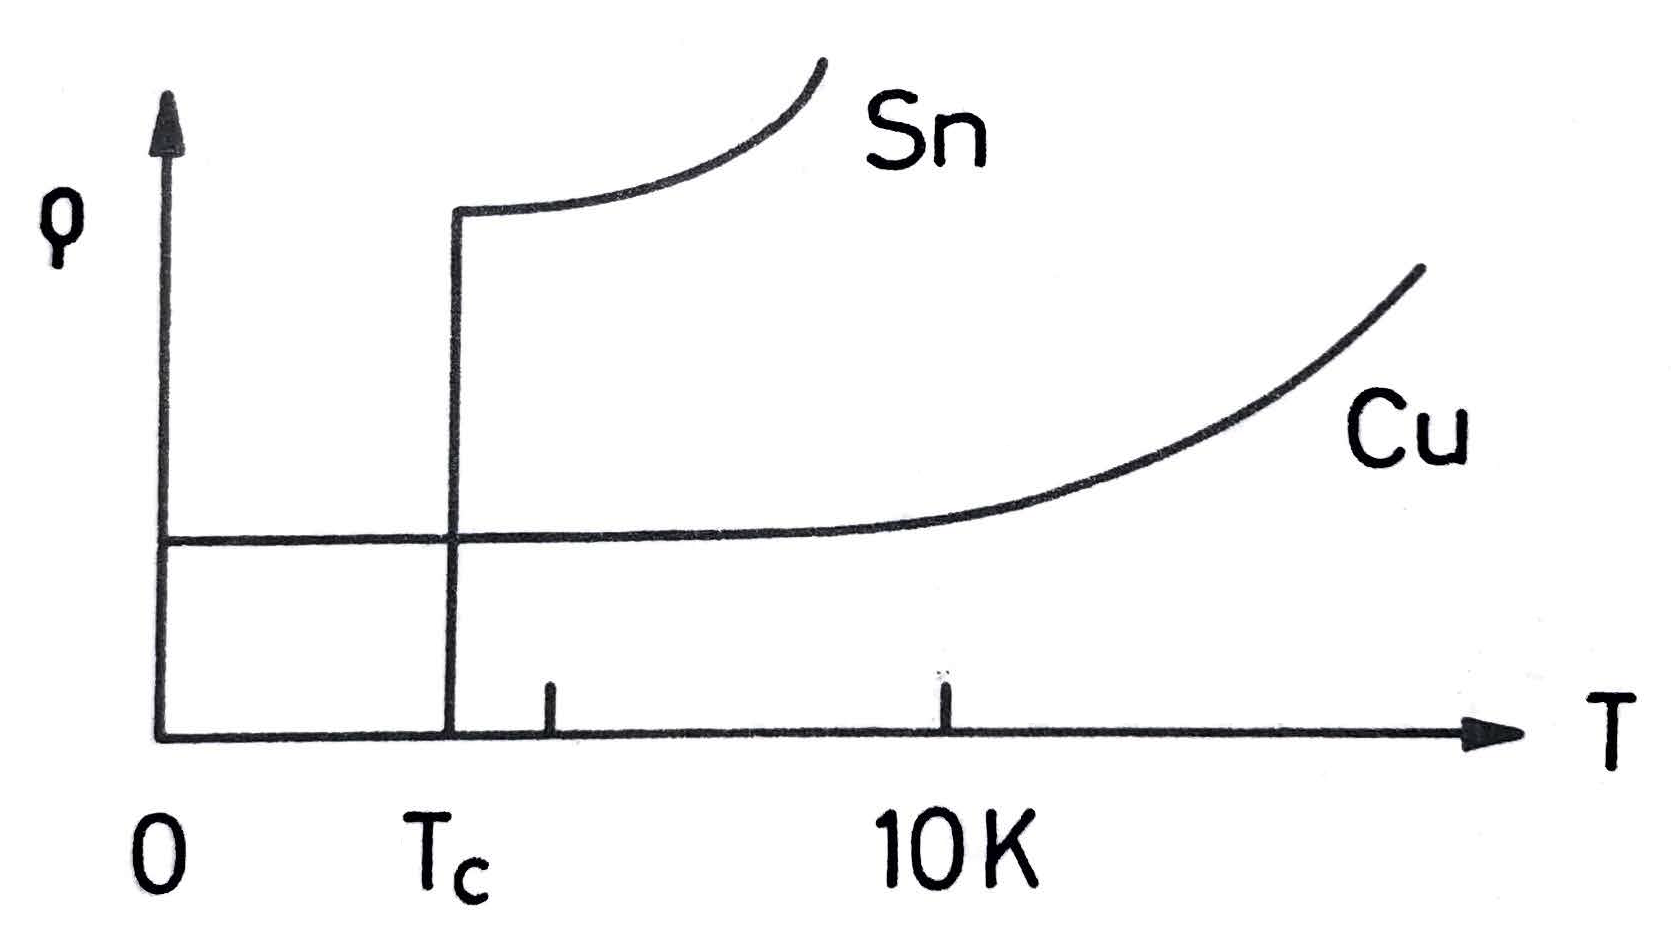
\includegraphics[width=0.35\linewidth]{sections/introduction/figures/sn_cu_resistivity.png}
    \caption{Resistivity of copper and tin at low temperatures~\cite{superconducting_accelerator_magnets}.}
    \label{fig:resitivity_tin_copper}
\end{figure} 

A superconductor is embedded in a~copper matrix which serves for three purposes~\cite[p.~31-33]{superconducting_accelerator_magnets}:

\begin{enumerate}
    \item Copper improves the mechanical properties of a superconductor such as mechanical strength and ductility.
    \item When a~superconductor quenches, the current starts commuting in both components of the composite strand. Copper, which is characterised by a~lower resistivity in a~normal conducting state with respect to the superconductor, enables most of the current current to bypass the superconductor.
    \item Copper increases the thermal stability of a superconductor by working as a heat sink. 
\end{enumerate}

Starting from the left picture in Fig.~\ref{fig:strand_and_filaments}, one can observe the groups of superconductor filaments. The diameter of a single filament is usually approximately equal to $10~\upmu$m. The picture in the middle represents a cross-section of a strand with multiple groups of filaments marked in grey that are embedded in a copper matrix. The diameter of a single strand usually accounts for 1~mm. The superconducting coil of a magnet can be either wound with strands or with Rutherford cables (picture in the right) that are a set of twisted strands. The Rutherford cable allows for limiting eddy currents in the copper matrix. The composite fabrication should ensure a good contact between the~copper and a~superconductor. The~copper should also be characterised by a high residual resistivity ratio (see Appendix~\ref{appendix:subsection_rrr_definition}), i.e. it ought to be highly conductive both electrically and thermally~\cite[p.~31-33]{superconducting_accelerator_magnets}.

\begin{figure}[H]
    \centering
    \begin{tikzpicture}
    \node at (10,0) {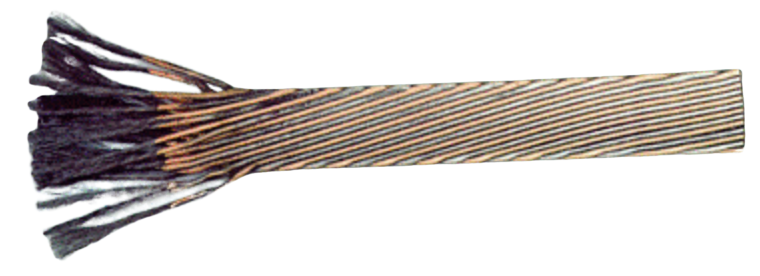
\includegraphics[width=.4\textwidth]{sections/introduction/figures/rutherford_cable.png}};
    \node at (4.4,0) {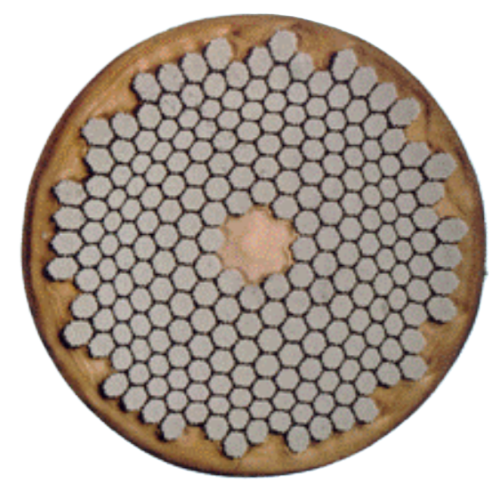
\includegraphics[width=.3\textwidth]{sections/introduction/figures/strand_cross_section.png}};
    \node at (0,0) {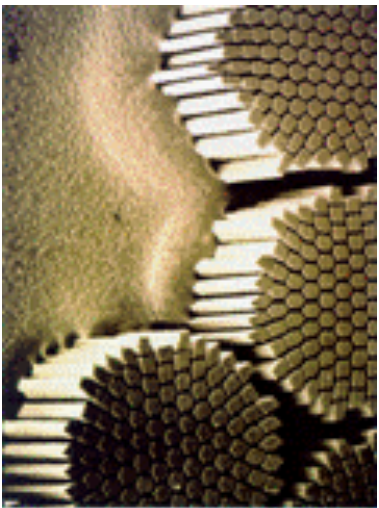
\includegraphics[width=.22\textwidth]{sections/introduction/figures/strand_filaments.png}};
    \end{tikzpicture}
    \caption{Left: groups of filaments embedded in a copper matrix, centre: strand cross-section with multiple groups of filaments, right: Rutherford cable~\cite{lhc_machine_outreach}.}
    \label{fig:strand_and_filaments}
\end{figure}

The strand stability is also increased due to liquid helium whose main role is to cool down the magnet to its operating conditions. Liquid helium is characterised by a high heat capacity with respect to solids at operating temperatures of LTS magnets. By assuring a good thermal contact between the strand and the liquid, one can increase the system stability. However, in many applications the strand or a stack of strands is fully impregnated with a~polymer that does not enable helium to penetrate the copper matrix. In such a case, the direct contact between the liquid and the strand is negligible and cooling of a quenched zone is only possible through a longitudinal heat propagation along the strand~\cite[p.~122]{superconducting_accelerator_magnets}.

Taking into consideration a superconducting magnet as a whole, composed of multiple strands, it may quench because of, among many, three reasons: 
\begin{enumerate}
    \item A coil element can move in a stack of strands due to the action of Lorentz forces. The frictional movement between different windings would result in the generation of heat.
    \item A part of a particle beam may be deposited in the beam pipe which would lead to the creation of a particle shower and, thus, to the generation of heat as well. 
    \item A malfunction of a cryogenic system can also be the reason for quench of a superconducting magnet. 
\end{enumerate}

\subsection{Current Sharing Phenomenon}

When a strand operates at the critical surface of a superconductor, the current starts commuting in both elements of the composite. This phenomenon is called "current sharing". At this point, it is assumed that the superconductor carries the current of a critical value $I_\text{c}$ while the copper matrix bypasses the surplus of this value equal to $I-I_\text{c}$, where $I$ is the transport current in the strand. The strand components can be represented as a~parallel connection of two resistors~\cite[p.~119-121]{superconducting_accelerator_magnets}. By assuming a linear dependence of $I_\text{c}$ on temperature, the critical current can be calculated as
\begin{equation}
    I_\text{c} \approx I \cdot \frac{T-T_\text{cs}}{T_\text{c}-T_\text{cs}},
\end{equation}
where $T$ -- local temperature of the strand. If the local temperature $T$ is assumed to be equal to the operating bath temperature $T_0$, one can deduce the current sharing temperature as
\begin{equation}
    T_\text{cs} = T_\text{0} + (T_\text{c} - T_\text{0}) \cdot (1 - \frac{I}{I_\text{c}~T_0}).
\end{equation}
Therefore, the current in a copper matrix $I_\text{Cu}$ can be divided into three regimes as
\begin{equation}
    \left\{ \begin{array}{ lll }
    I_\text{Cu} = 0 & \text{for}~T < T_\text{cs}, \\ \\
    I_\text{Cu} = I - I_\text{c} & \text{for}~T_\text{cs} \leq T<T_\text{c},  \\ \\
    I_\text{Cu} = I & \text{for}~T_\text{c} \leq T.
    \end{array} \right.
    \label{eqn:current_sharing}
\end{equation}
Above the critical temperature $T_\text{c}$, the superconductor resistance is much larger than the one of copper. Therefore, it is assumed that the current only flows through a copper stabiliser and only this part of the strand contributes to the Joule heating. In order to deduce the~Joule effect in all operating regimes of the~strand, one needs to specify the~composite fractions of the~strand as 

\begin{equation}
    \left\{ \begin{array}{ll}
    r_\text{Cu/s-cond} = \frac{f_\text{Cu}}{f_\text{s-cond}} = \frac{A_\text{Cu}}{A_\text{s-cond}}\\ \\
    f_\text{Cu} + f_\text{s-cond} = 1,
    \end{array} \right.
    \label{eqn: non_super_to_super_ratio}
\end{equation}
where $f_\text{Cu}$ -- volumetric fraction of copper, $f_\text{s-cond}$ -- volumetric fraction of a superconductor, $A_\text{Cu}$ -- cross-sectional area of copper, $A_\text{s-cond}$ -- cross-sectional area of a superconductor. Based on (\ref{eqn:current_sharing}) and (\ref{eqn: non_super_to_super_ratio}), the heat source in the strand is formulated as 
\begin{equation}
    q_\text{Joule} = J_\text{strand}^2~\rho_\text{strand} = J_\text{Cu}^2~\rho_\text{Cu}~f_\text{Cu} = \frac{I_\text{Cu}^2}{f_\text{Cu}^2~A_\text{strand}^2}~\rho_\text{Cu}~f_\text{Cu} = \frac{I_\text{Cu}^2}{A_\text{strand}^2}~\frac{\rho_\text{Cu}}{f_\text{Cu}}, 
    \label{eqn: p_dens_equiv}
\end{equation}
where $J_{strand}$ -- transport current density in a strand, $\rho_\text{strand}$ -- resistivity of a strand, $J_\text{Cu}$ -- current density in copper, $\rho_\text{Cu}$ -- resistivity of copper, $I_\text{Cu}$ -- current in a copper stabiliser, $A_\text{strand}$ -- cross-sectional area of a strand. One should notice that the copper resistivity $\rho_\text{Cu}$ should be divided by the non-superconductor fraction as 
\begin{equation}
    \rho_\text{strand} = \frac{\rho_\text{Cu}}{f_\text{Cu}}.
    \label{eqn:strand_resistivity}
\end{equation}

\subsection{Minimum Propagating Zone}

This section is based on~\cite[p.~124]{superconducting_accelerator_magnets}, and presents the analysis of a fully insulated strand in which the influence of helium in quench propagation is negligible. In the given consideration, the following assumptions are made: 
\begin{itemize}
    \item The strand is only made of a superconductor without a copper stabiliser. 
    \item The current density in the wire is close to its critical value. 
    \item The length $L$ of a superconductor is heated from the bath temperature $T_0$ to the temperature $T$ above the critical value $T_\text{c}$.
\end{itemize}

Since helium is not considered, the thermal disturbance in the strand leads to the~quench propagation if the longitudinal heat evacuation is lower than the generation of heat in the~quenched zone. It is formulated as
\begin{equation}
    \rho J^2 A L \geq \frac{kA(T_\text{c}-T_0)}{L},
\end{equation}
where $\rho$ -- resistivity of a superconductor, $J$ -- transport current density, $A$ -- wire cross-section, $L$ -- heated length of a superconductor, $k$~-- thermal conductivity of a superconductor. One can simply deduce the minimum propagating zone from the~equation as
\begin{equation}
    L_\text{MPZ} = \sqrt{\frac{2k(T_\text{c}-T_0)}{\rho J^2}}.
\end{equation}
If the thermal disturbance is larger or equal to $L_\text{MPZ}$, the quench starts propagating along the wire. For pure Nb-Ti, the $L_\text{MPZ}$ is approximately equal to $L=1~\upmu \text{m}$. Such a~small value explains why a~copper stabiliser is necessary in a composite strand. The usage of copper may increase $L_\text{MPZ}$ by a factor of thousand. 





